\documentclass[conference]{IEEEtran}
\IEEEoverridecommandlockouts

\usepackage{cite}
\usepackage{amsmath,amssymb,amsfonts}
\usepackage{algorithmic}
\usepackage{graphicx}
\usepackage{textcomp}
\usepackage{xcolor}
\usepackage{url}
\usepackage{hyperref}
\usepackage[T1]{fontenc}
\usepackage[utf8]{inputenc}
\usepackage[ngerman]{babel}

\def\BibTeX{{\rm B\kern-.05em{\sc i\kern-.025em b}\kern-.08em
    T\kern-.1667em\lower.7ex\hbox{E}\kern-.125emX}}
\begin{document}

\title{Covidash -- Dokumentation der Software-Architektur\\
{\footnotesize Web-Anwendungsentwicklung Sommersemester 2021}}
\author{
\IEEEauthorblockN{Bauer Tobias}
\textit{t.bauer@oth-aw.de}
\and
\IEEEauthorblockN{Hahn Albert}
\textit{a.hahn@oth-aw.de}
\and
\IEEEauthorblockN{Kleinlein Lukas}
\textit{l.kleinlein@oth-aw.de}
\and
\IEEEauthorblockN{Proske Nicolas}
\textit{n.proske@oth-aw.de}
\and
\IEEEauthorblockN{Wöllmer Leonard}
\textit{l.woellmer@oth-aw.de}
}

\maketitle

\begin{abstract}
    In dieser Dokumentation wird die Architektur des Projekts \textit{Covidash} von Team Weiß erläutert.
    Dabei wird auf die Lösungsstrategie mit besonderem Augenmerk auf den technologischen Aufbau eingegangen.
    Anschließend werden Schwierigkeiten während der Entwicklung sowie deren Lösungen aufgezeigt und ein abrundendes Fazit mit Ausblick gezogen.
\end{abstract}





\section{Problemstellung}



\subsection{Mission Statement}

Seit Beginn der Corona-Pandemie gilt es, der Bevölkerung die Informationen und aktuellen Kennzahlen geeignet darzustellen. Mit sich fast täglich ändernden politischen Regelungen und Restriktionen ist es für Privatpersonen wichtig, diese Informationen und Werte regelmäßig abzurufen.

Die Motivation hinter dem hiermit vorgestellten Covid-Dashboard ist es, dem Benutzer eine persönlich anpassbare Ansicht bereitzustellen, die seinen Informationsbedürfnissen entspricht. Hier liegt ein besonderes Augenmerk auf der räumlichen Relevanz, da sich die meisten Benutzer nur für die Kennzahlen einiger ausgewählter Landkreise (v.a. ihren Wohn- sowie Arbeitsort) interessieren.

Neben den aktuellen Inzidenz-Zahlen ist auch der Impffortschritt in Deutschland von großem Interesse, um den Schutz vor der Krankheit und möglichen Mutationen einschätzen zu können. Deshalb besteht das Dashboard aus zwei Hauptbestandteilen, dem Infektionsdashboard und dem Impfdashboard.

Entscheidend für die Benutzerfreundlichkeit ist zudem die Aktualität der Daten. Ziel von Covidash ist es, die Daten tagesaktuell abzurufen und darzustellen.



\subsection{Kontextabgrenzung}

Covidash bezieht Daten aus mehreren Quellen und stellt diese dem Benutzer aggregiert bereit.
Die folgende Abbildung~\ref{abb:blackbox} zeigt die Interaktionen des Systems mit Fremdsystemen und dem Benutzer.
\begin{figure}[htb]%
    \centering%
    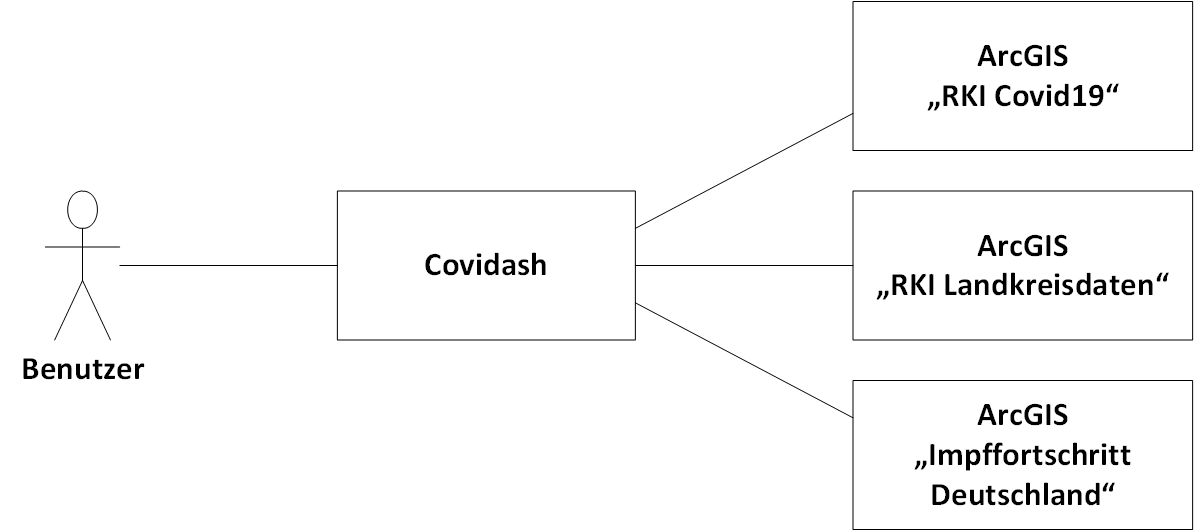
\includegraphics[width=0.76\columnwidth]{img/Kontextabgrenzung.png}%
    \caption{Visualisierung des Systems als Blackbox}%
    \label{abb:blackbox}%
\end{figure}

\vfill\eject

\subsection{Architekturziele}%
%
\begin{table}[h!]%
    \centering%
    \caption{}%
    \label{tab:architekturziele}%
    \def\arraystretch{1.5}%
    \begin{tabular*}{\columnwidth}{@{ }p{0.28\columnwidth}@{ }p{0.68\columnwidth}}%
        \textbf{Architekturziel} & \textbf{Motivation}\\
        \hline
        \hline
        Geographische Darstellung & Intuitive Ansicht in Form einer Landkarte führt zu besserer Verständlichkeit\\
        \hline
        Anpassbarkeit & Individualisierung durch den Benutzer erlauben, sodass der Fokus auf dessen relevante Daten gelegt werden kann\\
        \hline
        Tagesaktualität & Teils rapide Schwankungen der Werte und darauffolgende sofortige Konsequenzen im Alltag für den Benutzer erfordern regelmäßige Updates\\
        \hline
        Feine Granularität & Corona-Regelungen werden meist auf der kleinsten administrativen Ebene wirksam\\
        \hline
        Performance & Kurze Ladezeiten sorgen für einen schnellen Überblick\\
    \end{tabular*}
\end{table}






\section{Lösungsstrategie}

\subsection{Systemüberblick}

\begin{figure}[htb]%
    \centering%
    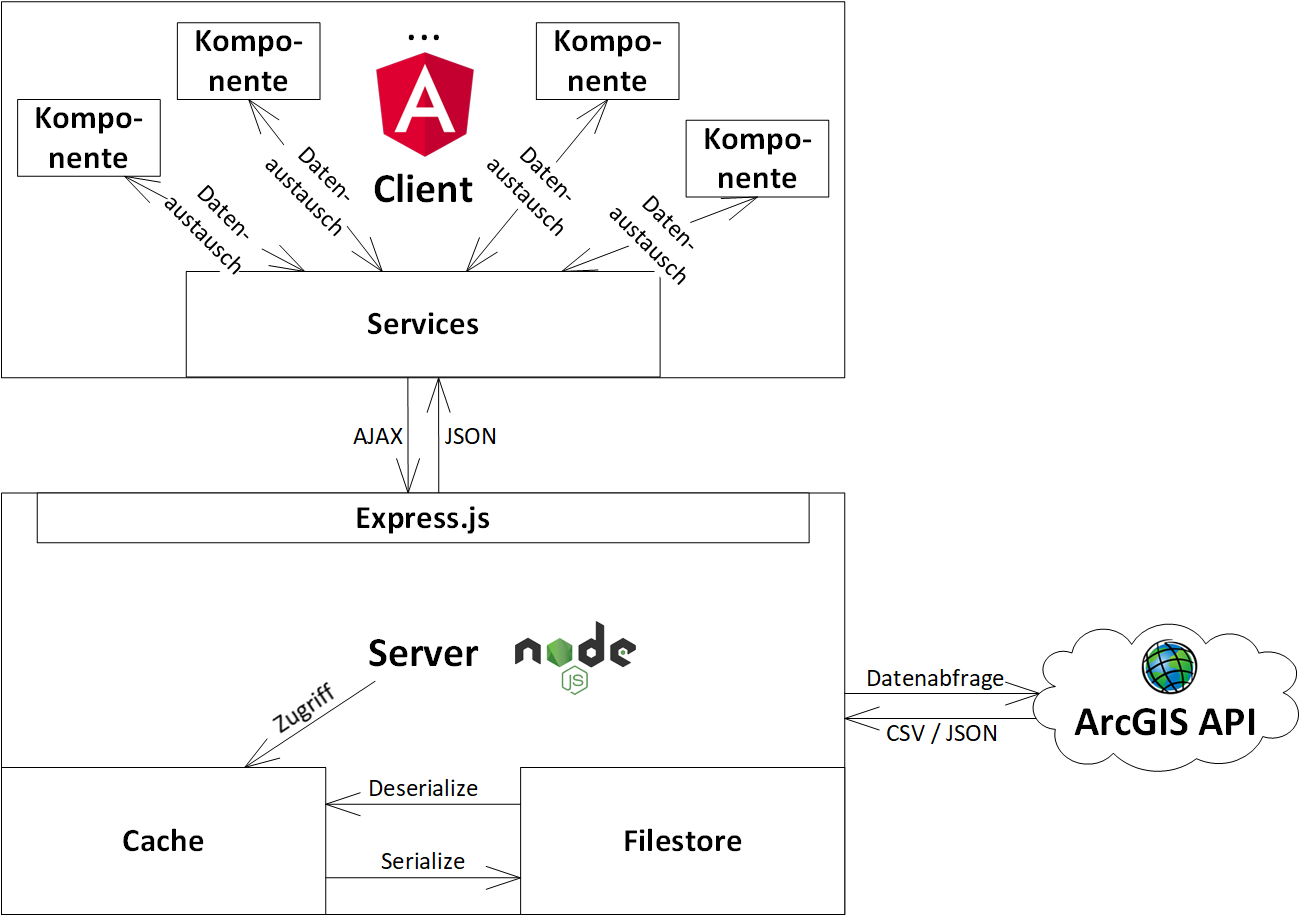
\includegraphics[width=0.95\columnwidth]{img/TechnologieStackLogo.png}%
    \caption{Aufbau des Systems + Externe API}%
    \label{abb:aufbau}%
\end{figure}
Covidash nutzt eine abgewandelte Version des MEAN-Stacks. Es wird auf den Einsatz einer MongoDB verzichtet, und stattdessen ein eigener Cache mit Filestore implementiert. Der Vorteil hiervon ist, dass alle Daten aggregiert im Arbeitsspeicher vorliegen. Somit entfallen jegliche Datenbank\-abfragen und die Antwortzeit des Backends verringert sich drastisch.



\subsection{Architektur Backend}

Covidash basiert auf den Daten des Robert-Koch-Instituts, welche über die öffentliche, von ArcGIS zur Verfügung gestellte, API bezogen werden. Zur Vereinheitlichung der Daten, welche aus unterschiedlichen Quellen stammen, werden sie über ein eigenes Backend aufbereitet. Im Anschluss werden diese über eine REST-Schnittstelle zur Verfügung gestellt.

Das Backend ist in TypeScript implementiert und läuft in einer Node.js-Umgebung.
Um die API-Routen zu definieren, wird das Framework Express.js verwendet.

Wenn eine Anfrage an das Backend gestellt wird, prüft der Server, ob die gewünschten Daten bereits im Arbeitsspeicher-Cache vorliegen. Ist dies der Fall, kann die Anfrage sofort beantwortet werden. Andernfalls wird versucht, auf den lokalen Filestore zuzugreifen, um die Daten zu laden und den Cache zu füllen. Gibt es keine zugehörige Datei, müssen die Daten neu bezogen und aufbereitet werden.

Hierfür wird eine Anfrage an die jeweils passende Rohdaten-API des RKIs gestellt. Die für Covidash relevanten Daten werden zunächst aus der Antwort extrahiert. Anschließend werden Transformationen und Aggegationen auf die gewonnenen Datensätze angewendet. Die fertig aufbereiteten Daten werden im lokalen Dateisystem gespeichert und zusätzlich im Arbeitsspeicher gecacht. Somit liegen sowohl im Cache als auch im Filestore die relevanten Daten immer aggregiert und strukturiert vor.
Zusätzlich werden die Infektionsrohdaten, die im CSV-Format vorliegen, als Backup abgespeichert.

Einmal täglich wird der lokale Datenstand als veraltet markiert. Mit der nächsten Anfrage sichert der Server den letzten Datenstand und bezieht neue Daten von den Rohdaten-APIs, um aktuell zu bleiben. Um den Festplattenspeicher des Servers nicht unnötig zu füllen, werden die alten Dateien mithilfe des Node-Packages \texttt{7zip-min}\cite{7zm} in ein Archiv gepackt und komprimiert. Die Daten werden wie oben beschrieben im lokalen Dateisystem abgelegt und in den Cache geladen.

Die folgende Tabelle~\ref{tab:routen} schlüsselt alle Routen auf, die das Backend zur Verfügung stellt. Eine Anfrage erfolgt immer an die Adresse der Form \texttt{https://covidash.de/api/<Route>}.
\newline
Um beispielsweise eine Anfrage für die aktuellen Impf- und Inzidenzwerte Deutschlands zu stellen, ist folgende Adresse aufzurufen: \texttt{https://covidash.de/api/summary}.
\begin{table}[h!]%
    \centering%
    \def\arraystretch{1.5}%
    \caption{}%
    \label{tab:routen}%
    \begin{tabular*}{\columnwidth}{@{ }p{0.33\columnwidth}@{ }p{0.63\columnwidth}}%
        \textbf{Route} & \textbf{Beschreibung}\\
        \hline
        \hline
        /incidences/<county-id> & Infektions-Daten für den Landkreis mit der ID <county-id>\\
        \hline
        /incidences/0           & Infektions-Daten für ganz Deutschland\\
        \hline
        /incidences/diff        & Die Änderungen der Inzidenzen zum vorigen Datenelement (für alle Landkreise in ganz Deutschland)\\
        \hline
        /incidences             & Die neusten Inzidenzen aller Landkreise\\
        \hline
        /counties               & Namen aller Landkreise und ihre IDs\\
        \hline
        /vaccines/<stateId>     & Impfdaten pro Bundesland\\
        \hline
        /vaccines/diff          & Die Änderungen der Impfdatenstände zum vorigen Datenelement (für alle Bundesländer in ganz Deutschland)\\
        \hline
        /vaccines               & Die neusten Impfdaten aller Bundesländer\\
        \hline
        /summary                & Aktuelle Impf-- \& Inzidenzwerte Deutschlands\\
        \hline
        /summary/diff           & Die Änderungen der Impf-- \& Inzidenzwerte Deutschlands zum vorigen Datenelement
    \end{tabular*}
    \vspace{0.1cm}
\end{table}



\subsection{Architektur Frontend}

Aufseiten des Clients kommt das Framework Angular zum Einsatz.

Auf die vom Backend bereitgestellten Schnittstellen wird über die mit Angular realisierte Web-Anwendung mithilfe von Services zugegriffen und die Daten werden bei Bedarf an die jeweiligen Komponenten weitergegeben.
Durch die Verwendung dieser Services wird doppelter Code vermieden und eine einheitliche Handhabung der Daten gewährleistet.

Insgesamt gibt es vier Services, welche in die zwei folgenden Kategorien unterteilt werden können: Services mit und ohne Kommunikation mit dem Backend. Unter Erstere fallen die „Infections“- und „Vaccines“-Services, welche sich grundlegend um das Laden und Aufbereiten der empfangen Daten für die einzelnen Komponenten kümmern. Zu dieser Kategorie gehört ebenfalls der „Network“-Service, welcher alle Funktionen für die Netzwerkabfragen bereitstellt. Der „Favorite“-Service ist der zweiten Kategorie zuzuordnen und neben der Bereitstellung eines „Favoriten teilen“-Links auch für die zentrale Verwaltung der Favoriten zuständig.

In der Web-Anwendung kann über die „Dashboard wechseln“-Funktion zwischen den zwei Seiten Infektions\-dashboard und Impfdashboard hin- und hergewechselt werden. Umgesetzt wurde diese Funktion mittels Angular-Routing, wodurch man über bestimmte URLs auf festgelegte Komponenten verweisen kann, welche der Benutzer schlussendlich angezeigt bekommt. Dies wurde auch dazu verwendet, um die URL-Parameter des automatisch erzeugten „Favoriten teilen“-Links auslesen zu können. Der Nutzer wird durch eine spezielle URL auf eine bestimmte Komponente weitergeleitet, welche beim Aufruf die URL-Parameter ausliest und über den „Favorite“-Service im LocalStorage des Browsers abspeichert.

Um ähnliche Oberflächenkomponenten nicht doppelt implementieren zu müssen bauen sich die oben erwähnten Seiten aus vielen unterschiedlichen Angular-Komponenten zusammen -- ein Beispiel hierfür wäre die „Map“-Komponente, welche sowohl auf dem Infektionsdashboard als auch auf dem Impfdashboard zur interaktiven Anzeige der Infektions- bzw. Impfdaten dient.

Über den Node.js-Paketmanager \texttt{npm}\cite{npm} können externe Module, sogenannte „node modules“, in das Projekt eingebunden werden. Mit Hilfe dieser Open-Source-Bibliotheken kann das Projekt schnell und einfach um weitere Funktionalitäten erweitert werden. Diese Module sind über die komplette Anwendung nutzbar. Die bereits erwähnte „Map“-Komponente nutzt beispielsweise zur Darstellung der Karte das Modul \texttt{Leaflet}\cite{Leaflet}.

SCSS ist die in der Web-Anwendung eingesetzte Stylesheet-Sprache, womit intelligente Syntax geschrieben werden kann, um die übliche Komplexität von CSS beherrschen zu können und den Code übersichtlich zu halten. Die Dateien der Style-Kategorien „Colors“ und „Responsiveness“ wurden in eigene Unterdateien ausgelagert und mittels \texttt{@import}-Befehl in die Hauptdatei importiert.



\subsection{Hosting}

Zur Präsentation von Covidash wird die Web-Anwendung auf einem virtualisierten (Cloud-)Server mit 2 Kernen und 4 GB RAM unter der Verwendung von Debian 10 als Betriebssystem gehostet. Da es sich hierbei um keinen typischen Webspace handelt, mussten alle Vorbereitungen für das Hosting der eigentlichen Anwendung inklusive Backend selbst getroffen werden. Dazu zählen unter anderem die Installation eines Webservers für Front- und Backend, das Aufschalten einer Domain und die Konfiguration eines SSL-Zertifikats.

Nginx bietet die Möglichkeit, sogenannte Serverblöcke („server blocks“, vergleichbar mit „virtual hosts“ in Apache) zu erstellen, womit Konfigurationsdetails gekapselt werden können, sodass mehrere Websites auf einem Server parallel gehostet werden können. Demnach wurde für das Frontend ein eigener Serverblock –- unabhängig vom standardmäßig mitinstallierten Serverblock –- angelegt und so konfiguriert, dass alle Anfragen standardmäßig auf das Verzeichnis des Angular-Projekts weiterleiten, welches zum Aufruf des Frontends führt. Alle Anfragen mit \texttt{/api} in der URL werden an die Node.js-Umgebung mit entsprechendem Port weitergeleitet. Aufgrund der Verwendung des Prozessmanagers \texttt{pm2}\cite{pm2} muss die Node.js-Umgebung lediglich einmal gestartet werden und läuft ab da als eigene Instanz im Hintergrund weiter. Sollte sie abstürzen, kümmert sich \texttt{pm2} um einen automatischen Neustart.

Die Registrierung der Domain \texttt{covidash.de} erfolgte bereits vor der Einrichtung des Servers. Direkt nach Freischaltung der Domain wurden neue DNS-Records angelegt, welche die Domain auf die IPv4-Adresse des zuvor konfigurierten Servers weiterleiten.

Let's Encrypt ist eine Zertifizierungsstelle, die eine unkomplizierte Möglichkeit bietet, kostenlose TLS/SSL-Zertifikate zu erhalten und zu installieren, die verschlüsseltes HTTPS auf Webservern ermöglichen. Für die Konfiguration dieses Zertifikats wurde \texttt{certbot}\cite{certbot} verwendet, um ein kostenloses SSL-Zertifikat für die Domain \texttt{covidash.de} zu erhalten, welches sich zudem kurz vor Ablauf automatisch erneuert.






\section{Schwierigkeiten}

Bei der Umsetzung von Covidash taten sich einige Hürden auf, welche die Entwicklung erschwerten. Im Folgenden werden die gravierendsten Schwierigkeiten erläutert und deren Problemlösungen beschrieben.



\subsection{Hohe Arbeitsspeicherlast}

Die Entwicklung des Backends von Covidash fand auf herkömmlichen Dekstop-PCs unter Windows 10 statt. Nachdem lokale Tests erfolgreich absolviert worden waren, wurde der Quellcode auf den gemieteten Cloud-Server ausgerollt und dort ausgeführt. Zunächst war dieser nur mit 2~GB Arbeitsspeicher ausgestattet. Aufgrund der Datenmengen, die beim Parsen der heruntergeladenen Rohdaten-Datei anfiel, wurde die Node.js-Umgebung vom eingesetzten Linux-Betriebssystem zwangsweise beendet.

Der erste Lösungsansatz hierfür war es, mehr Arbeitsspeicher zu installieren. Im Folgenden wurde mit einem Server mit 4~GB RAM gearbeitet. Zudem musste die Größe der Auslagerungsdatei von 512~MB auf ebenfalls 4~GB erhöht werden, da weiterhin Fehler wegen des geringen verfügbaren Arbeitsspeichers auftraten.

Die bis jetzt beschriebene Lösung funktionierte solange, bis der Datenstand durch das tägliche Update zum ersten Mal automatisiert erneuert wurde. Beim Erneuern der Daten gab die Node.js-Umgebung den Arbeitsspeicher nicht wieder optimal frei, wodurch der Prozess abermals zwangsweise beendet wurde.

Um dieses Problem zu adressieren, musste die Garbage-Collection (GC) in der Node.js-Umgebung manuell angestoßen werden. Die Schnittstelle zur GC ist standardmäßig nicht verfügbar und muss mittels eines speziellen Arguments beim Starten der Umgebung explizit für den Laufzeit-Code freigeschalten werden. Problematisch hierbei ist, dass der eingesetzte Laufzeit-Compiler \texttt{ts-node}\cite{ts-node} die Weiterreichung von Kommandozeilenargumenten an die darunterliegende Node.js-Umgebung nicht unterstützt. Um diese Einschränkung zu umgehen, muss die Umgebung manuell gestartet und \texttt{ts-node} darüber ausgeführt werden. Das folgende Kommando startet das Backend über \texttt{pm2} und informiert Node.js zusätzlich über die Größe des verfügbaren Arbeitsspeichers:

\texttt{pm2 start node -{}-}

\texttt{-{}-expose-gc -{}-max-old-space-size=4096}

\texttt{node\_modules/ts-node/dist/bin server.ts}



\subsection{Probleme mit der Rohdaten-API}

Während der Entwicklung von Covidash traten zwei unterschiedliche Probleme im Zusammenhang mit den verwendeten APIs zutage.

Einerseits wurde die für die Gewinnung der Impffortschrittsdaten genutzte API in Teilen deaktiviert. Der Endpunkt war zwar noch verfügbar, jedoch wurden nur noch veraltete Daten zurückgeliefert. Da dies kein technischer Fehler war, fielen die Ungenauigkeiten erst eine Woche später und nach mehrmaligem Testen auf. Im Zuge dessen musste auf eine neuere Version der API umgestellt werden. Glücklicherweise war die Datenstruktur in großen Teilen identisch zur Vorversion -- nur einzelne Datenfelder wurden umbenannt.

Andererseits besteht ein grundsätzliches Problem in der Struktur der Infektionsdaten des RKIs. Bereits bestehende Datensätze werden im Nachhinein angepasst: Beispielsweise werden die Genesenen nicht als neuer Datensatz erfasst, sondern der Erkrankungsdatensatz modifiziert. Somit kann aus den Daten nicht errechnet werden, wie viele aktive Infektionsfälle zu einem beliebigen Zeitpunkt existierten. Lediglich die \textit{heute} aktiven Fälle können akkurat bestimmt werden.






\section{Fazit und Ausblick}

Covidash beinhaltet zwei Ansichten, die das Infektionsgeschehen und den Impffortschritt in Deutschland visualisieren. Beide Dashboards stellen die Daten jeweils interaktiv in Form einer Karte, mehrerer Diagramme und einer durchsuchbaren Übersichtstabelle dar. Durch die Auswahl eines Landkreises bzw. eines Bundeslandes werden die Diagramme automatisch mit den für dieses Gebiet geltenden Daten befüllt.

Zudem können Benutzer ohne vorherige Anmeldung die für sie relevanten Landkreise auswählen und als Favoriten speichern sowie teilen.

Durch die tägliche Aufbereitung der Rohdaten und das mehrstufige Caching-System können die tagesaktuellen Daten zuverlässig und schnell abgerufen werden. Zusammen mit der übersichtlichen, responsiven Oberfläche wird dadurch eine positive User-Experience erreicht.

Covidash stellt eine solide Infrastruktur dar, die auch im Falle anderer Epidemien oder Pandemien wiederverwendet werden könnte. Durch die strikte Trennung von Front- und Backend besteht darüber hinaus die Möglichkeit, andere API-Anbieter einzubinden. Auch die Caching-Funktionalität innerhalb des Backends ist unabhängig von den Daten und kann dementsprechend ebenfalls wiederverwendet werden.





\begin{figure*}[ht!]%
    \centering%
    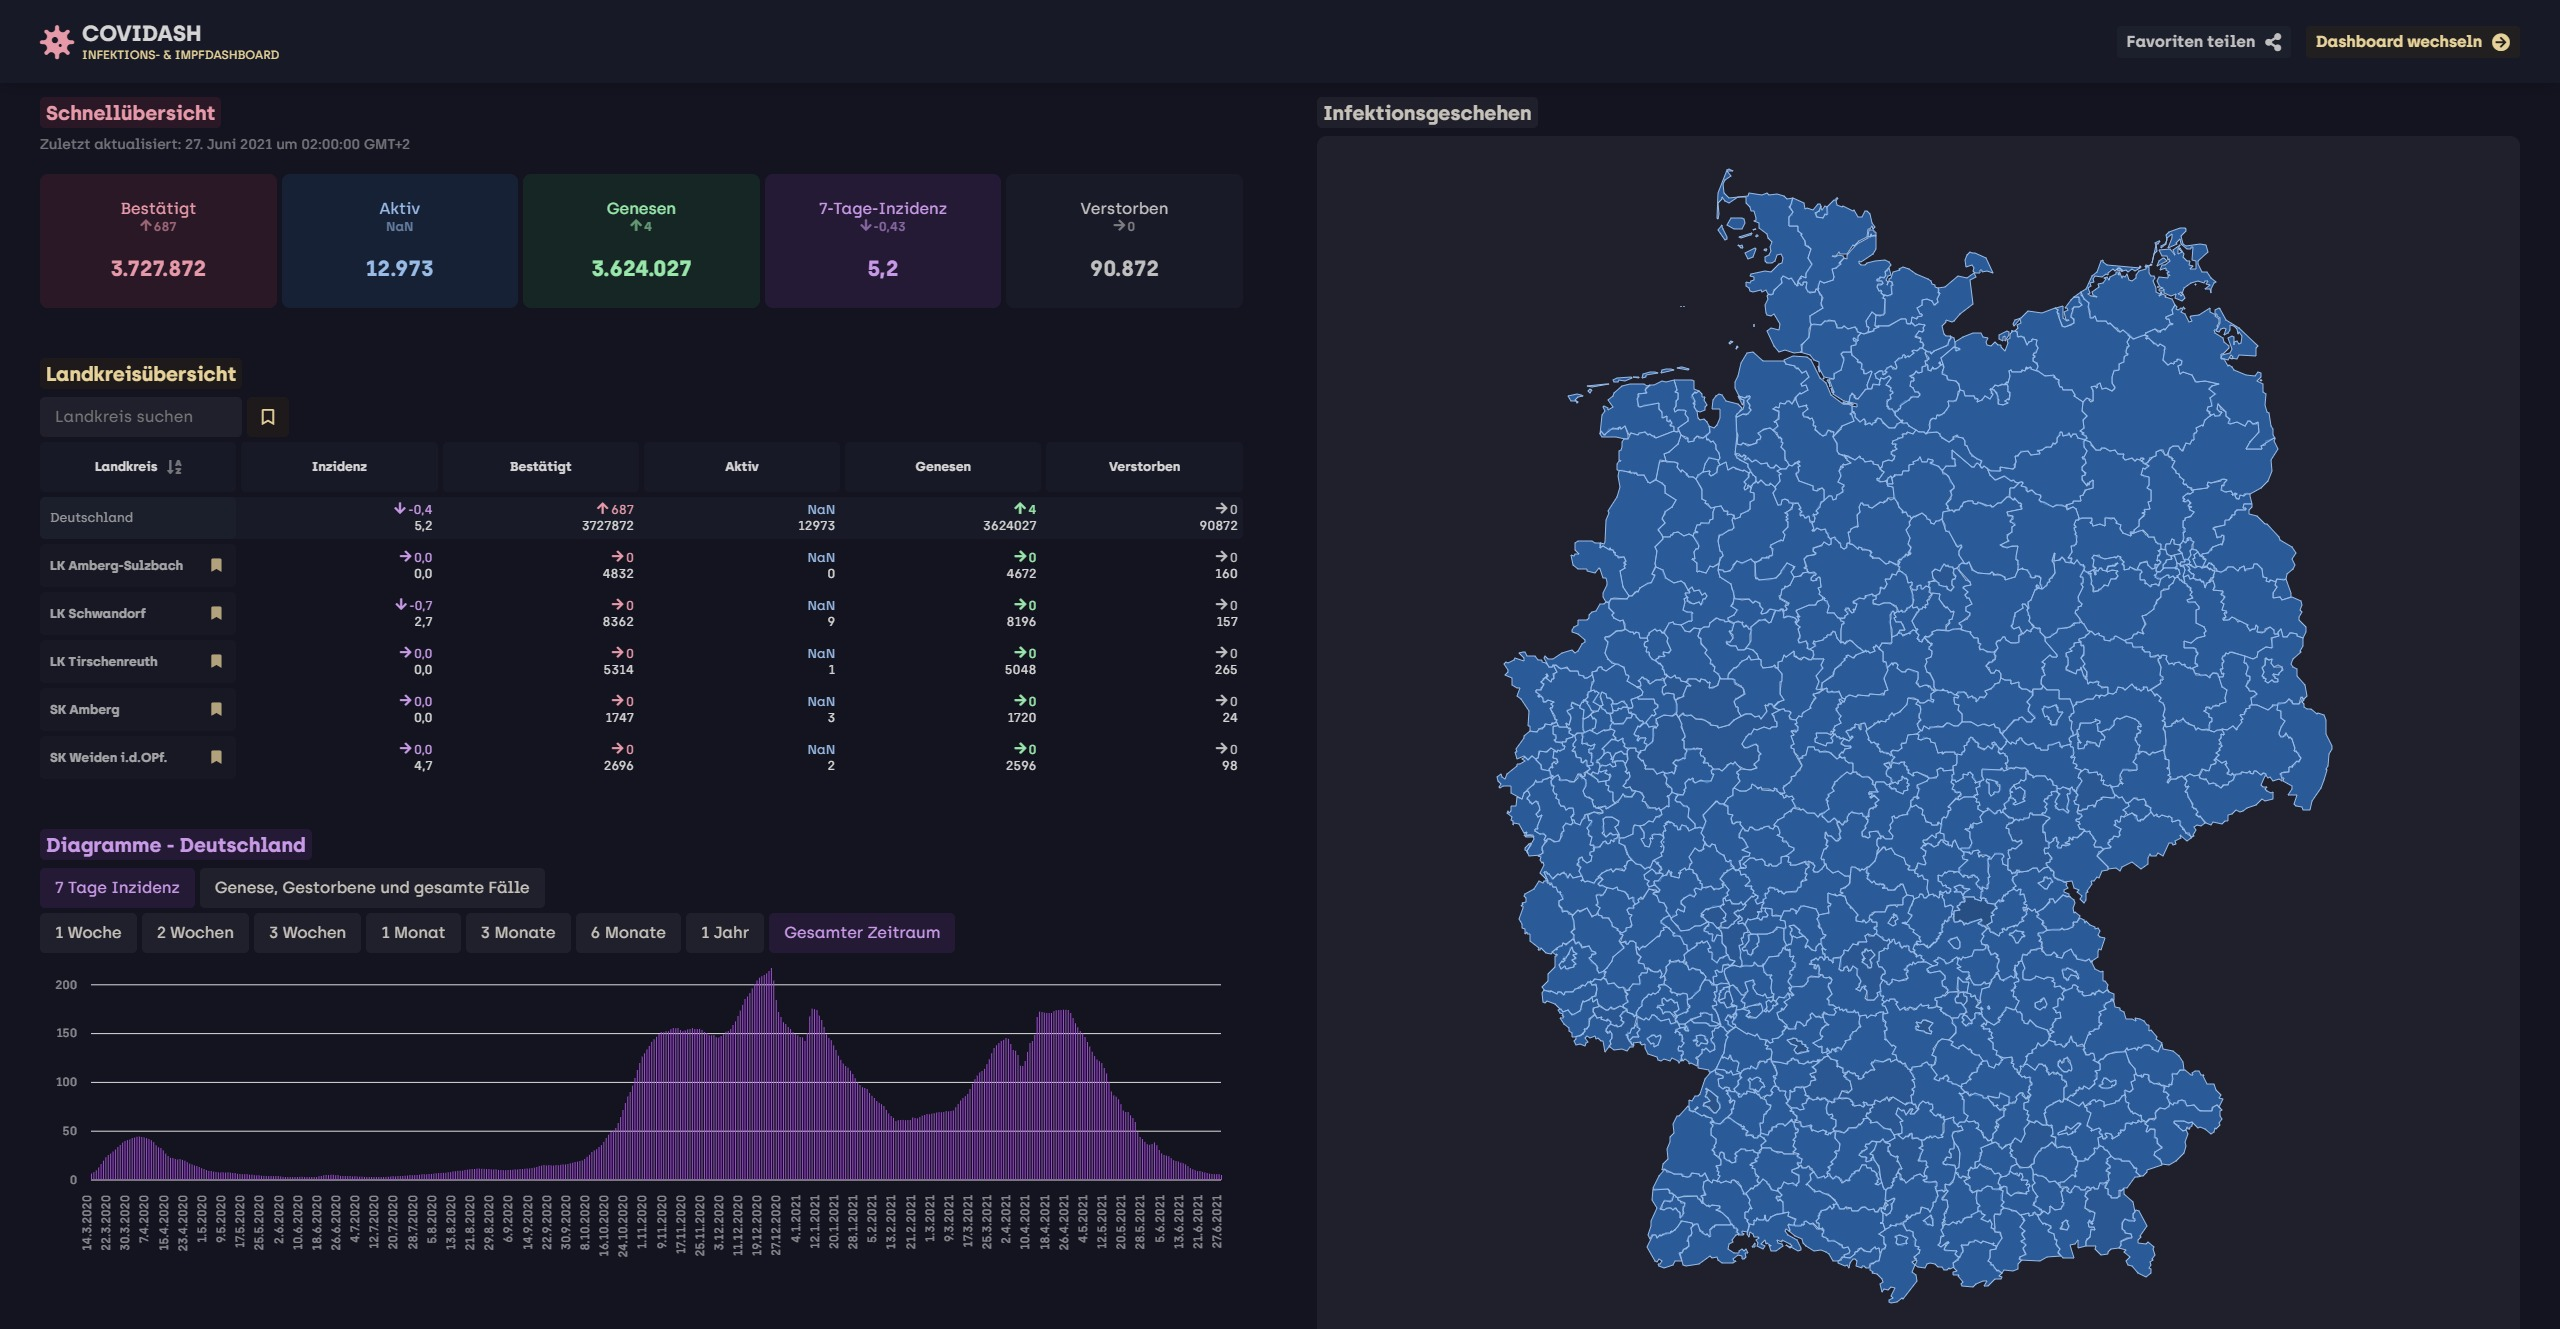
\includegraphics[width=0.96\textwidth]{img/screenshot_infections.jpg}%
    \caption{Screenshot der Website - Infektionsdaten}%
    \label{abb:screen_infections}%
\end{figure*}

\begin{figure*}[ht!]%
    \centering%
    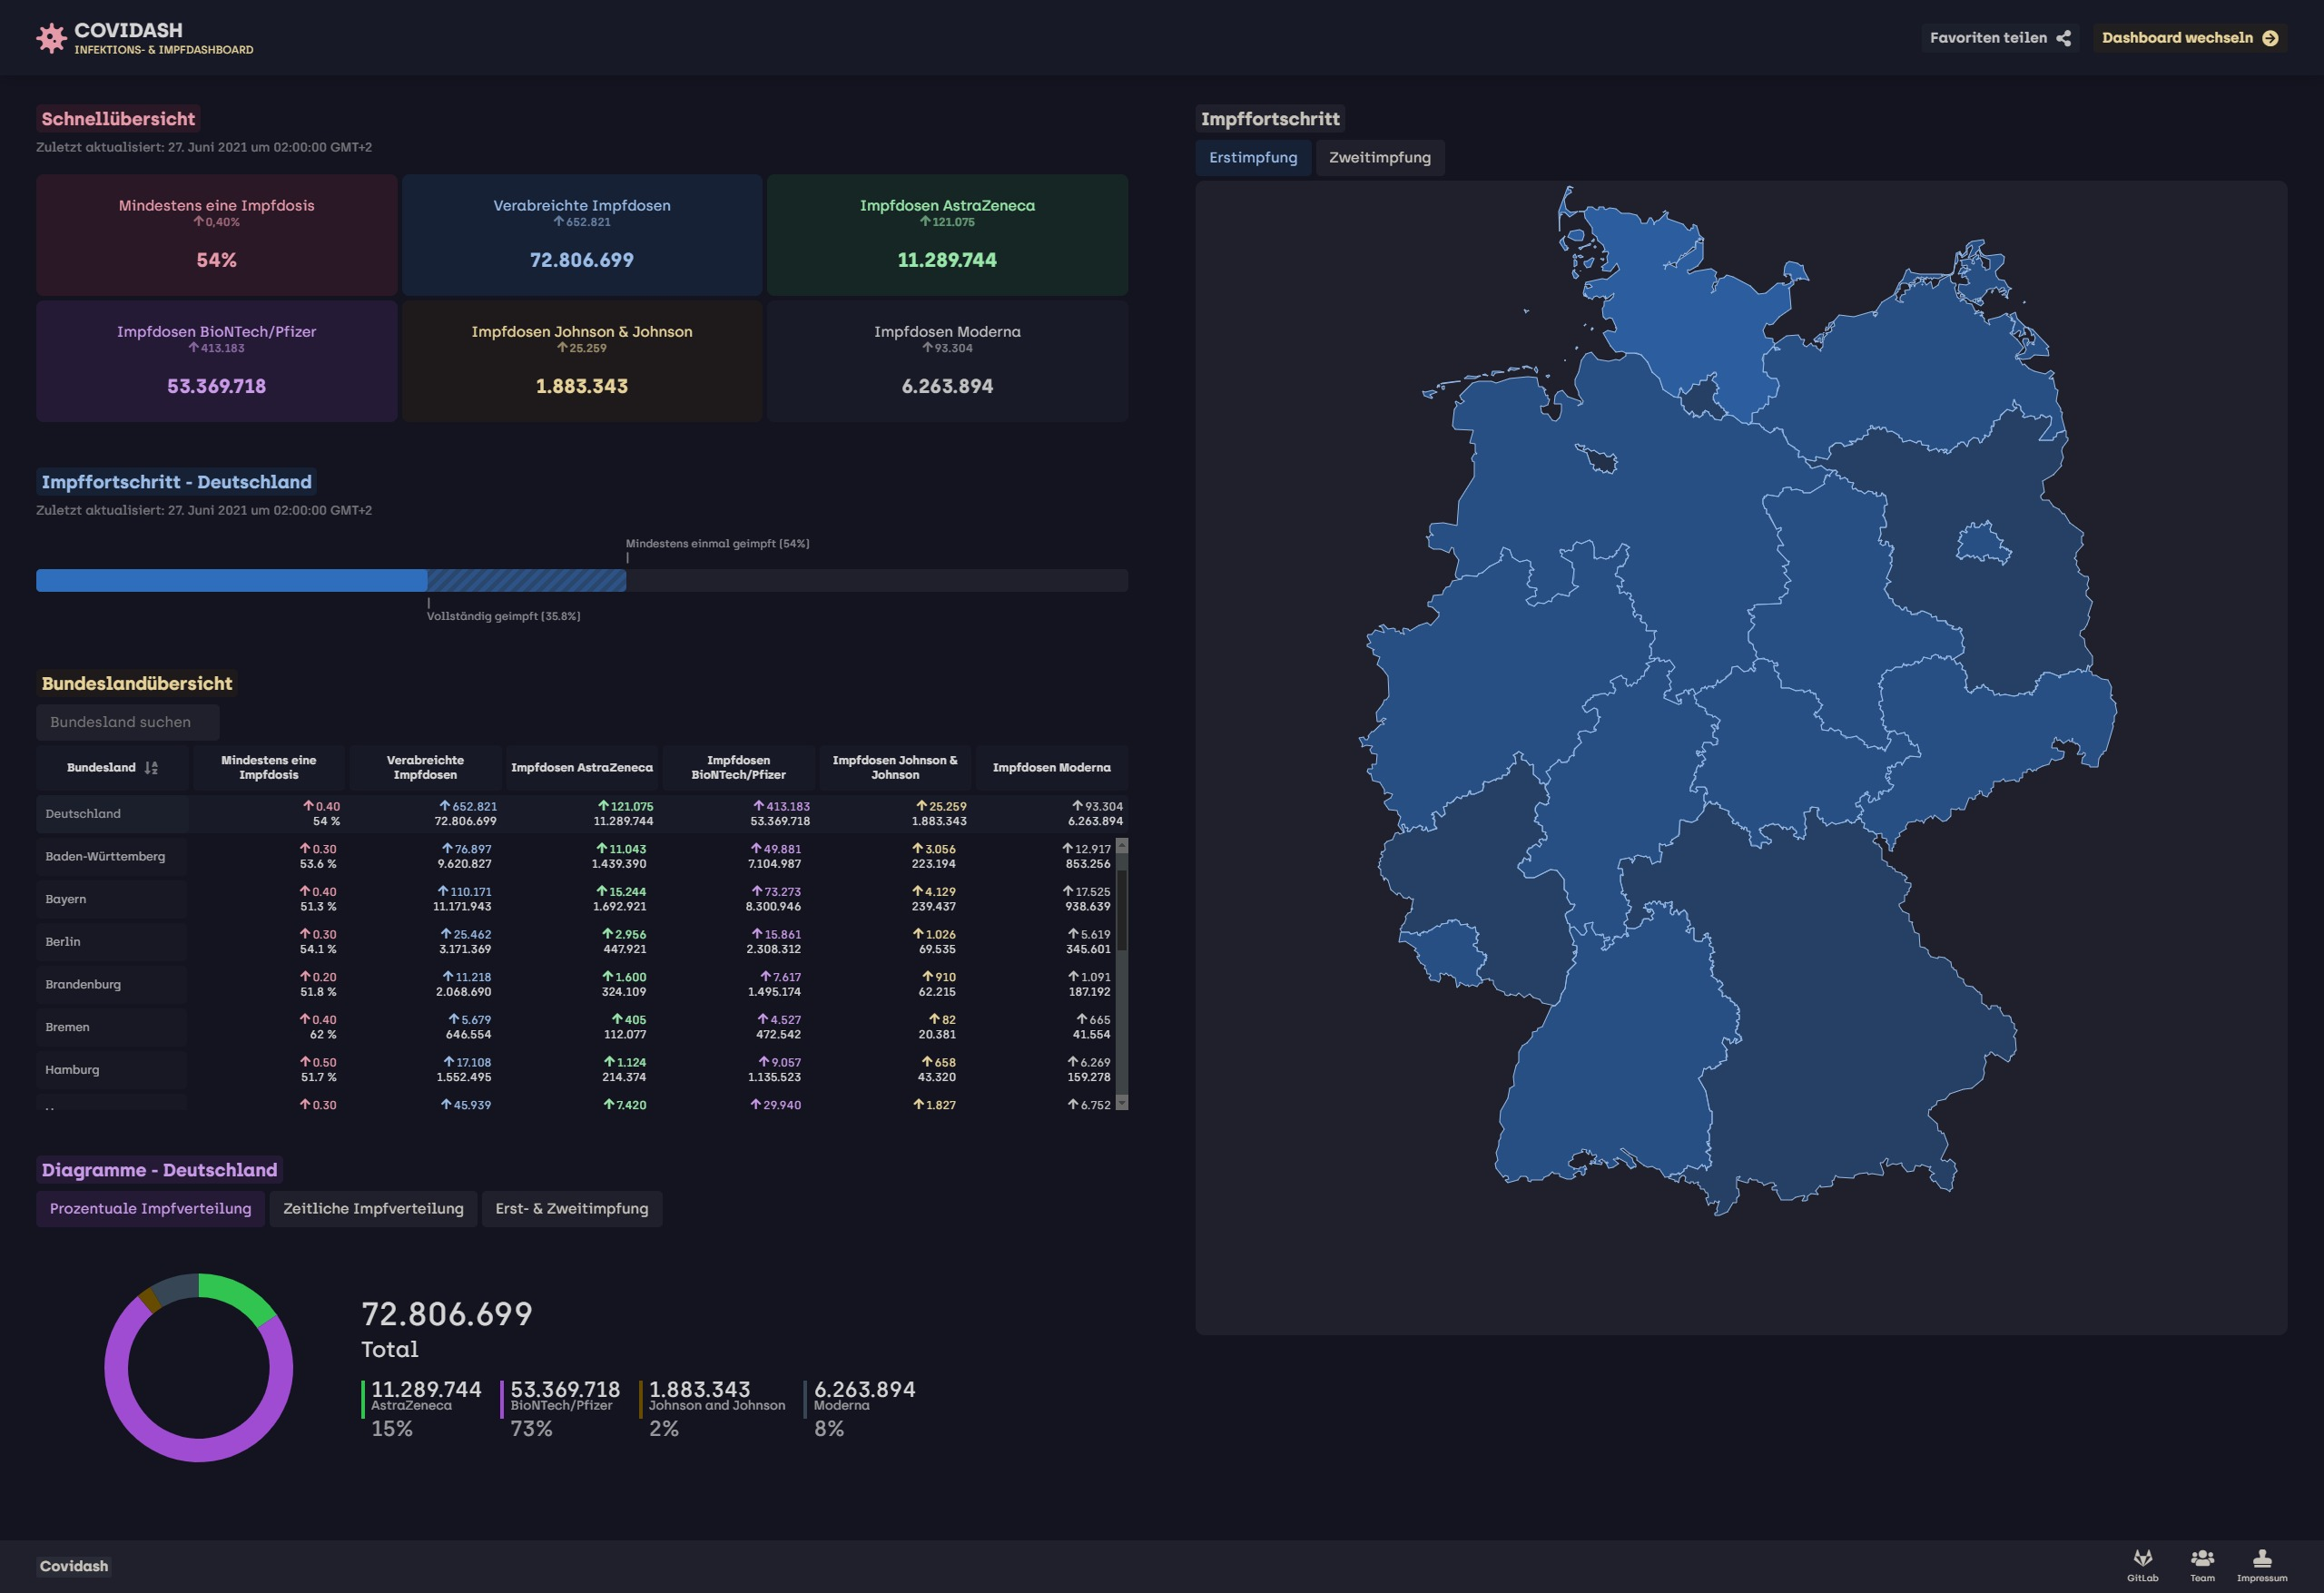
\includegraphics[width=0.96\textwidth]{img/screenshot_vaccines.jpg}%
    \caption{Screenshot der Website - Impfdaten}%
    \label{abb:screen_vaccines}%
\end{figure*}


\begin{thebibliography}{99}
    \bibitem{7zm} 7zip-min: https://www.npmjs.com/package/7zip-min
    \bibitem{npm} npm: https://www.npmjs.com/
    \bibitem{Leaflet} Leaflet: https://www.npmjs.com/package/leaflet
    \bibitem{pm2} pm2: https://www.npmjs.com/package/pm2
    \bibitem{certbot} certbot: https://certbot.eff.org/
    \bibitem{ts-node} ts-node: https://www.npmjs.com/package/ts-node
\end{thebibliography}

\end{document}